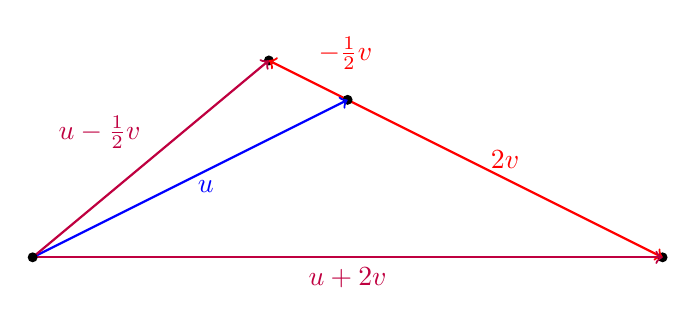
\begin{tikzpicture}[scale=2]
      \fill (1.5,1.25) circle (0.9pt);
      \fill (4,0) circle (0.9pt);
      \draw[->, thick, red] (2,1) -- node[above]{$\vect{2v}$} (4,0);
      \draw[->, thick, red] (2,1) -- node[above right]{$-\frac{1}{2}\vect{v}$} (1.5, 1.25);
      \fill (2,1) circle (0.9pt);
      \draw[->, thick, blue] (0,0) -- node[below,pos=0.55]{$\vect{u}$} (2,1);
      \draw[->, thick, purple](0,0) -- node[below]{$\vect{u}+2\vect{v}$} (4,0);
      \draw[->, thick, purple](0,0) -- node[above left]{$\vect{u} - \frac{1}{2}\vect{v}$} (1.5,1.25);
      \fill (0,0) circle (0.9pt);
    \end{tikzpicture}
